\chapter{The ATLAS Detector}

The \ac{ATLAS} detector is a cylindrical general purpose particle detector designed to measure the products of $\sqrt{s} = 14 \TeV$ proton-proton collisions at the \ac{LHC}. It consists of three major sub-detectors: closest to the beamline is the the \ac{ID}, which measures the trajectories of charge particles, followed by the Calorimeters, which measure the energies of electromagnetic and hadronically interacting particles, and finally the \ac{MS} which measures the trajectories of muons. The \ac{ID} is surrounded by a super conducting solenoidal magnet that provides a uniform $2\textrm{T}$ magnetic field, enabling measurement of particles' charge and momentum, and a toroidal magnet surrounds \ac{MS}, allowing for charge and momentum measurements of muons. In general, each subdetector consists of a barrel detector parallel to the beampipe and endcap detectors perpendicular to the beampipe.

A schematic of the \ac{ATLAS} detector is shown in \autoref{fig:atlas-schematic}.


%https://atlas.cern/discover/detector
\begin{figure}[htbp]
\centering
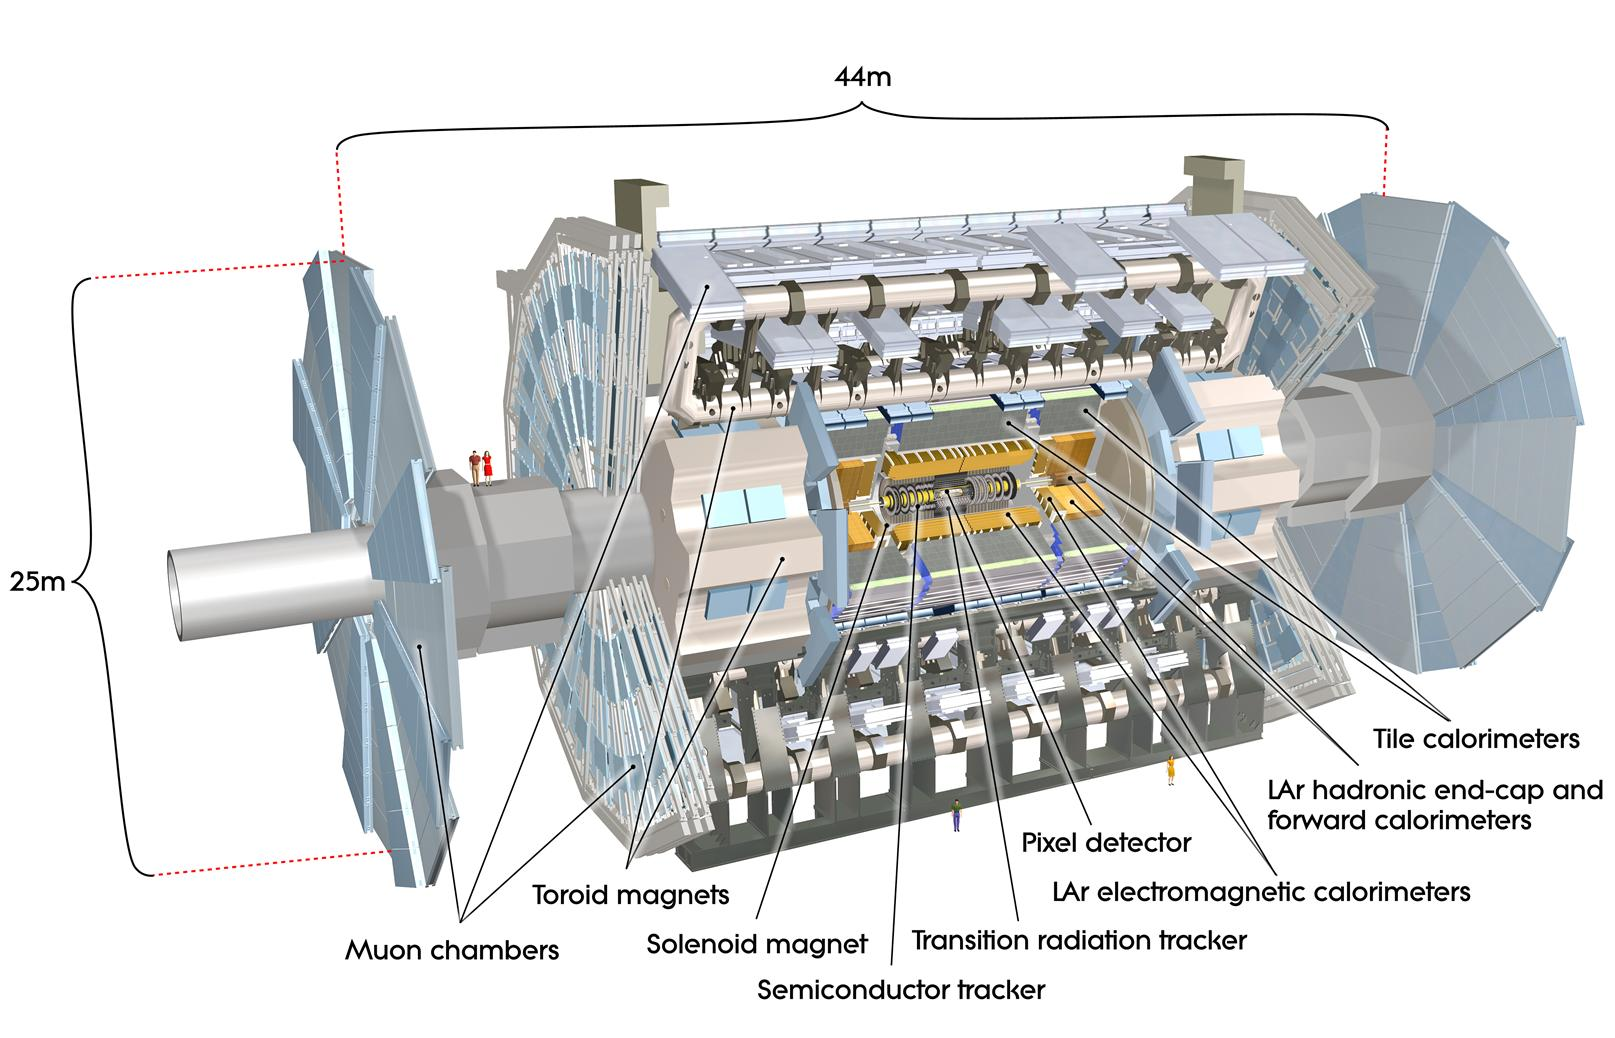
\includegraphics[width=.8\textwidth]{figures/Detector/atlas-schematic.jpg}
\caption{A diagram of the \ac{ATLAS} detector. The dimensions, subdetectors, and magnet systems are labeled. }
\label{fig:atlas-schematic}
\end{figure}

\section{Coordinate System}
\ac{ATLAS} uses a Cartesian right-handed coordinate system, with the origin defined as the $pp$ collision point. The $z$-axis points along the beampipe, where $+z$ points counter-clockwise. The transverse plane, the $y$-axis and $x$-axis, points upward and toward the center of the \ac{LHC} ring, respectively. The detector is built with with symmetry across the origin in in $z$, as well as with rotational symmetry in the transverse plane. The $+z$ side of the detector is referred to as the A-side, and $-z$ as the C-side.

Cylindrical coordinates provide a comfortable description of the \ac{ATLAS} detector, where $\phi$ measures the angle in the $x-y$ plane around the beampipe, and $\theta$ the angle from the $z$ axis. $\phi$ is positive for positive $y$. 

A given particle's momentum in $z$ is not known, but its transverse momentum is known to be $0$, so it is advantageous to define spatial variables independent of $z$ momentum. Thus, instead of $\theta$, $\eta = - \textrm{ln}(\textrm{tan}\frac{\theta}{2})$ is used to describe angle from the $z$ axis. Particles perpendicular to the $z$ axis have $\eta = 0$, while those parallel to the beamline have $\eta \rightarrow \infty$. 

Angular distances between objects is described using $\Delta R = \sqrt{\Delta \eta ^2 + \Delta \phi ^2}$ and the radial distance from the origin in the $x-y$ plane is denoted $R$. 

A particle's momentum will generally be described in terms of its \pT, its momentum in the transverse direction. A particle's $3$-vector is described by $(\pt, \eta, \phi)$, which are all invariant under boosts in $z$ assuming the particle can be considered massless (which is true in the case of particles in \ac{ATLAS}).






\section{Inner Detector}
The Inner Detector measures the trajectories of charged particles resulting from \ac{LHC} collisions. The \ac{ID} covers the region with $|\eta| < 2.5$, measuring approximately $1000$ particles per bunch crossing. In order to achieve the momentum and vertex resolution required to achieve \ac{ATLAS}'s physics goals three subdetectors are used: the Pixel detector, the \ac{SCT}, and the \ac{TRT}. The Pixel and \ac{SCT} detectors are used for high granularity precision tracking and the \ac{TRT} is used to distinguish electrons from converted photons. All of this is immersed in a $2T$ magnetic field, curving charged particles in proportion to its momentum.

\todo{describe conversions somewhere... Maybe in particle descriptions in theory?}


The \pt resolution of the \ac{ID} scales with track \pt. Higher \pt tracks are less curved, so the measurement resolution is worse. In the \ac{ATLAS} \ac{ID}, the \pt resolution  $0.05\% \times \pt$ with a $1\%$ constant term. The constant term describes measurement uncertainties that do not scale with momentum or energy, such as material imperfections, non-uniform detector response, or other constant measurement issues and is added in quadrature ($\oplus$) with the stochastic term.



A schematic of the \ac{ID} can be seen in \autoref{fig:atlas-id} and a detailed distribution of the various subdetectors is shown in \autoref{fig:atlas-id-layers}. 


%https://cds.cern.ch/images/CERN-GE-0803014-01/file?size=medium
\begin{figure}[htbp]
\centering
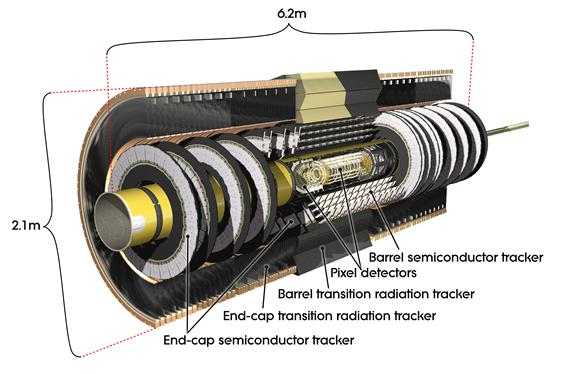
\includegraphics[width=.8\textwidth]{figures/Detector/atlas-ID.jpg}
\caption{A diagram of the \ac{ATLAS} \ac{ID} with the major subsystems labeled. The Pixel and \ac{SCT} are of particular importance for this analysis.}
\end{figure}

%https://www.researchgate.net/publication/325643426/figure/fig8/AS:669532737769482@1536640452588/Segment-of-the-ATLAS-inner-detector-showing-the-tracker-layers-The-silicon-strip.ppm
\begin{figure}[htbp]
\centering
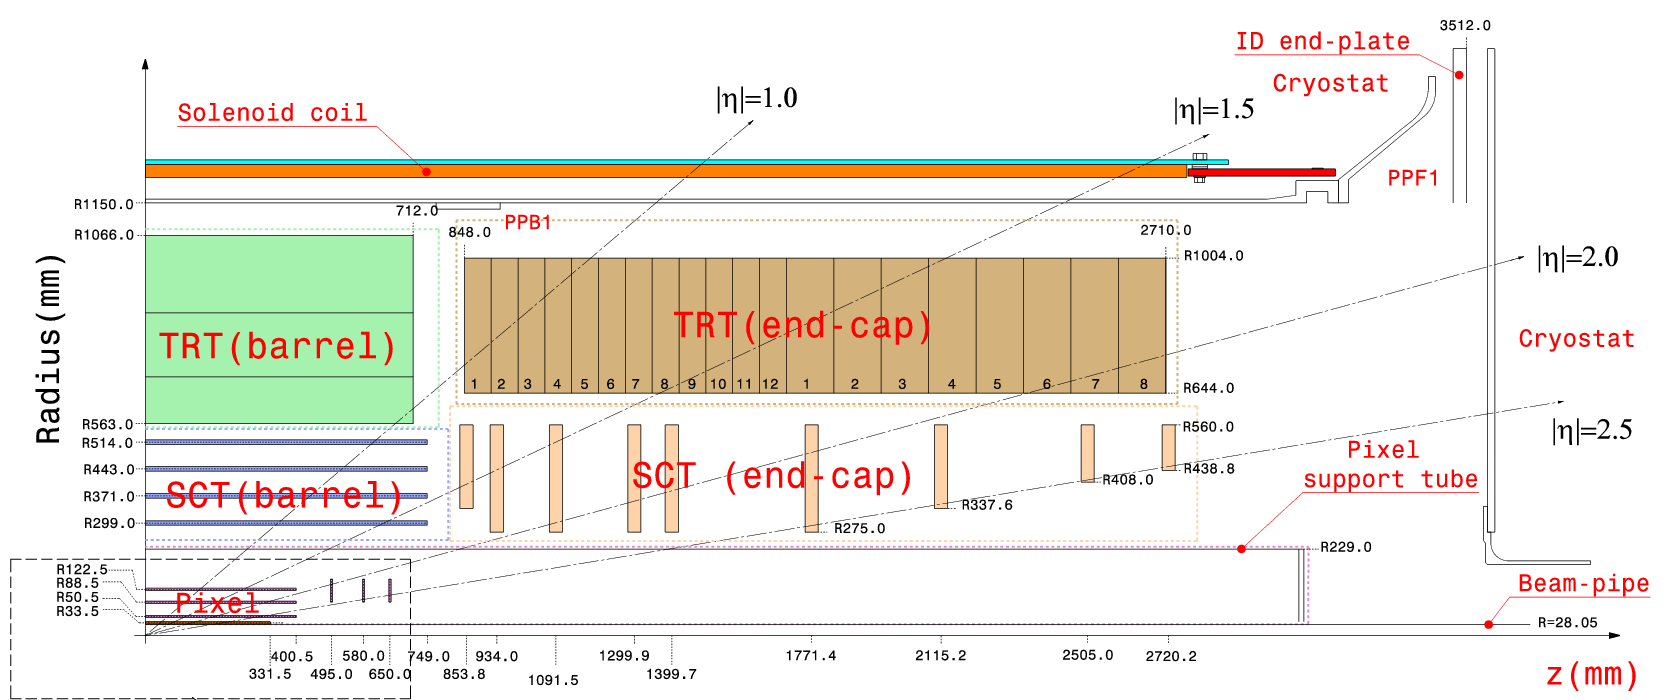
\includegraphics[width=.8\textwidth]{figures/Detector/atlas-id-layers.png}
\caption{A schematic of the \ac{ATLAS} \ac{ID} shown in the $r-z$ plane. }
\label{fig:atlas-id-layers}
\end{figure}

\subsection{The Pixel Detector}
\subsubsection{Hit Reconstruction}
\subsection{The Silicon Microstrip Tracker}
\subsubsection{Hit Reconstruction}
\subsection{The Transition Radiation Tracker}


\section{Calorimeters}

The \ac{ATLAS} calorimeters measure the energy of electromagnetic and hadronic particles. The \ac{LAr} electromagnetic sampling calorimeter is the innermost calorimeter and gives excellent energy and position resolution, with energy resolution of $10\%/\sqrt{E} \oplus $ in the region with $|\eta| < 3.2$. The hadronic scintillator-tile calorimeter surrounds the \ac{LAr} and gives $50\%/\sqrt{E} \oplus 3\%$ energy resolution in the region with $|\eta| < 3.2$. Additional \ac{EM} and hadronic calorimeters in the forward region extend coverage to $|\eta| < 4.9$, but with worse energy resolution ($100\%/\sqrt{E} \oplus 10\%$). Unlike the tracker, the energy resolution of a calorimeter increases with increasing energy due to the increased signal generated. A schematic of the \ac{ATLAS} calorimeters can be seen in \autoref{fig:atlas-calos}. 


%https://arxiv.org/pdf/1603.02934.pdf
\begin{figure}[htbp]
\centering
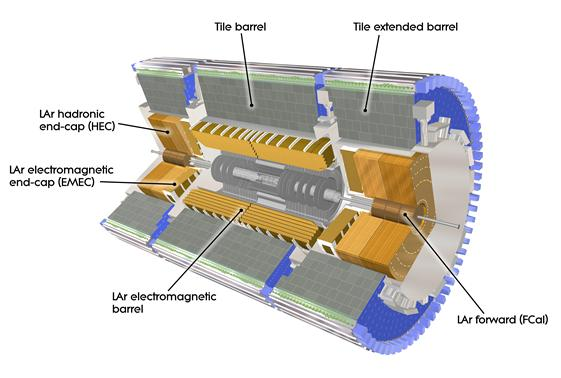
\includegraphics[width=.8\textwidth]{figures/Detector/atlas-calorimeters.jpg}
\caption{A diagram of the \ac{ATLAS} calorimeters with the major subsystems labeled. The \ac{LAr} is of particular importance for this analysis.}
\label{fig:atlas-calos}
\end{figure}


\subsection{Electromagnetic Calorimeter}

\subsection{Hadronic Calorimeter}


\section{Muon Spectrometer}
The Muon Spectrometer is the outermost subdetector designed to measure muons, which are too massive to be stopped by the \ac{LAr}. The \ac{MS} relies on a air-core toroidal magnet system which provide a strong bending power without introducing extra material scattering. It includes three layers of high precision tracking, which give a momentum resolution of $10\%$ at $\pT > 1 \TeV$ \footnote{At high \pt, the \ac{MS} performance is independent of the \ac{ID} resolution.} and separate trigger chambers with timing resolution of $1.5-4 \textrm{ns}$. 

%$https://cds.cern.ch/record/1631701/files/MuonSpectrometer_profile.png
\begin{figure}[htbp]
\centering
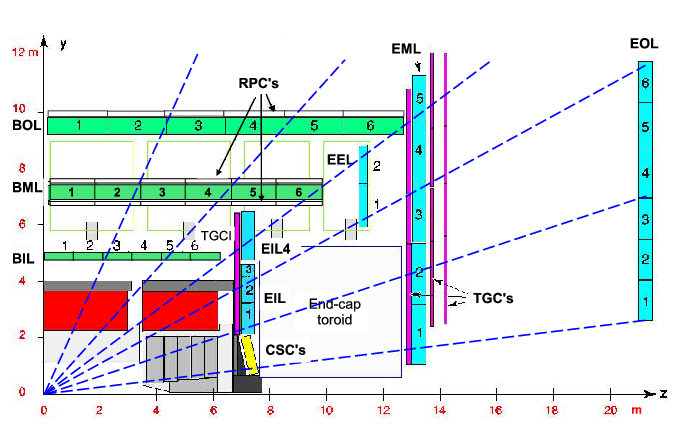
\includegraphics[width=.8\textwidth]{figures/Detector/atlas-ms.png}
\caption{A diagram of the \ac{ATLAS} \ac{MS} in the $r-z$ plane. The barrel \ac{MDT} are shown in green and the \ac{RPC} shown in black. In the endcaps, the \ac{MDT} are shown in blue and the \ac{TGC} shown in purple. }
\label{fig:atlas-ms}
\end{figure}


\section{Magnet Systems}
\label{sec:magnets}

\section{Particles in ATLAS}
The previously described subdetectors are used in combination to identify particles in \ac{ATLAS}. Charged particles interact with the \ac{ID} resulting in hits to be reconstructed into tracks. A track that points to a calorimeter cluster indicates the kind of charged particle that made the track and a cluster without an associated track indicates a neutral particle. The calorimeters are designed such that they absorb all of the energy of a particle and \ac{EM} particles do not enter the hadronic calorimeter, and hadronic particles do not enter the \ac{MS}. Muons do not interact with the calorimeters, but do leave a track in both the \ac{ID} and \ac{MS}. The only \ac{SM} particle that escapes the detector entirely is a neutrino. An undetected particle, like an \ac{SM} $\nu$ or some \ac{BSM} particle, could be seen as an imbalance in transverse momentum. The transverse momenta of all particles should sum to zero in order to conserve momentum, so any non-zero sum indicates an undetected particle.


\begin{figure}[htbp]
\centering
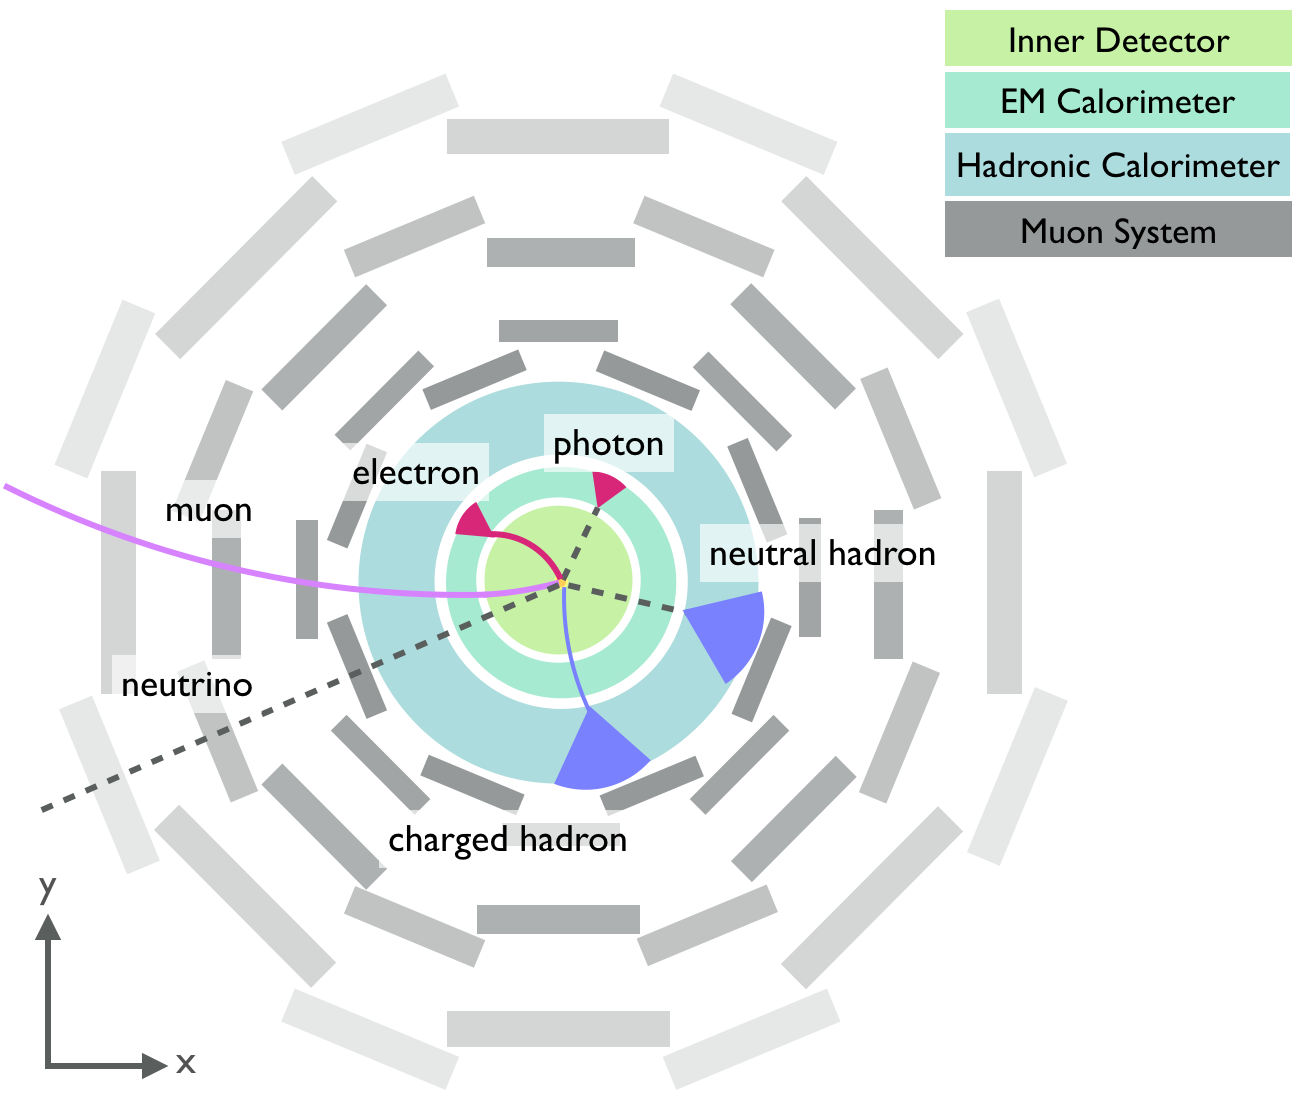
\includegraphics[width=.8\textwidth]{figures/Detector/particle-doodle.png}
\caption{A schematic of the signatures of Standard Model particles in the \ac{ATLAS} detector that illustrates how the subdetectors are used together to identify particles. Dashed lines indicate a particle trajectory that leaves no detector signature. Figure not drawn to scale nor does it represent a real physical process at the \ac{LHC}. }
\label{fig:particle-doodles}
\end{figure}




